\begin{figure*}[t]
\centering
\IfFileExists{figures/study_area_ramis.png}{%
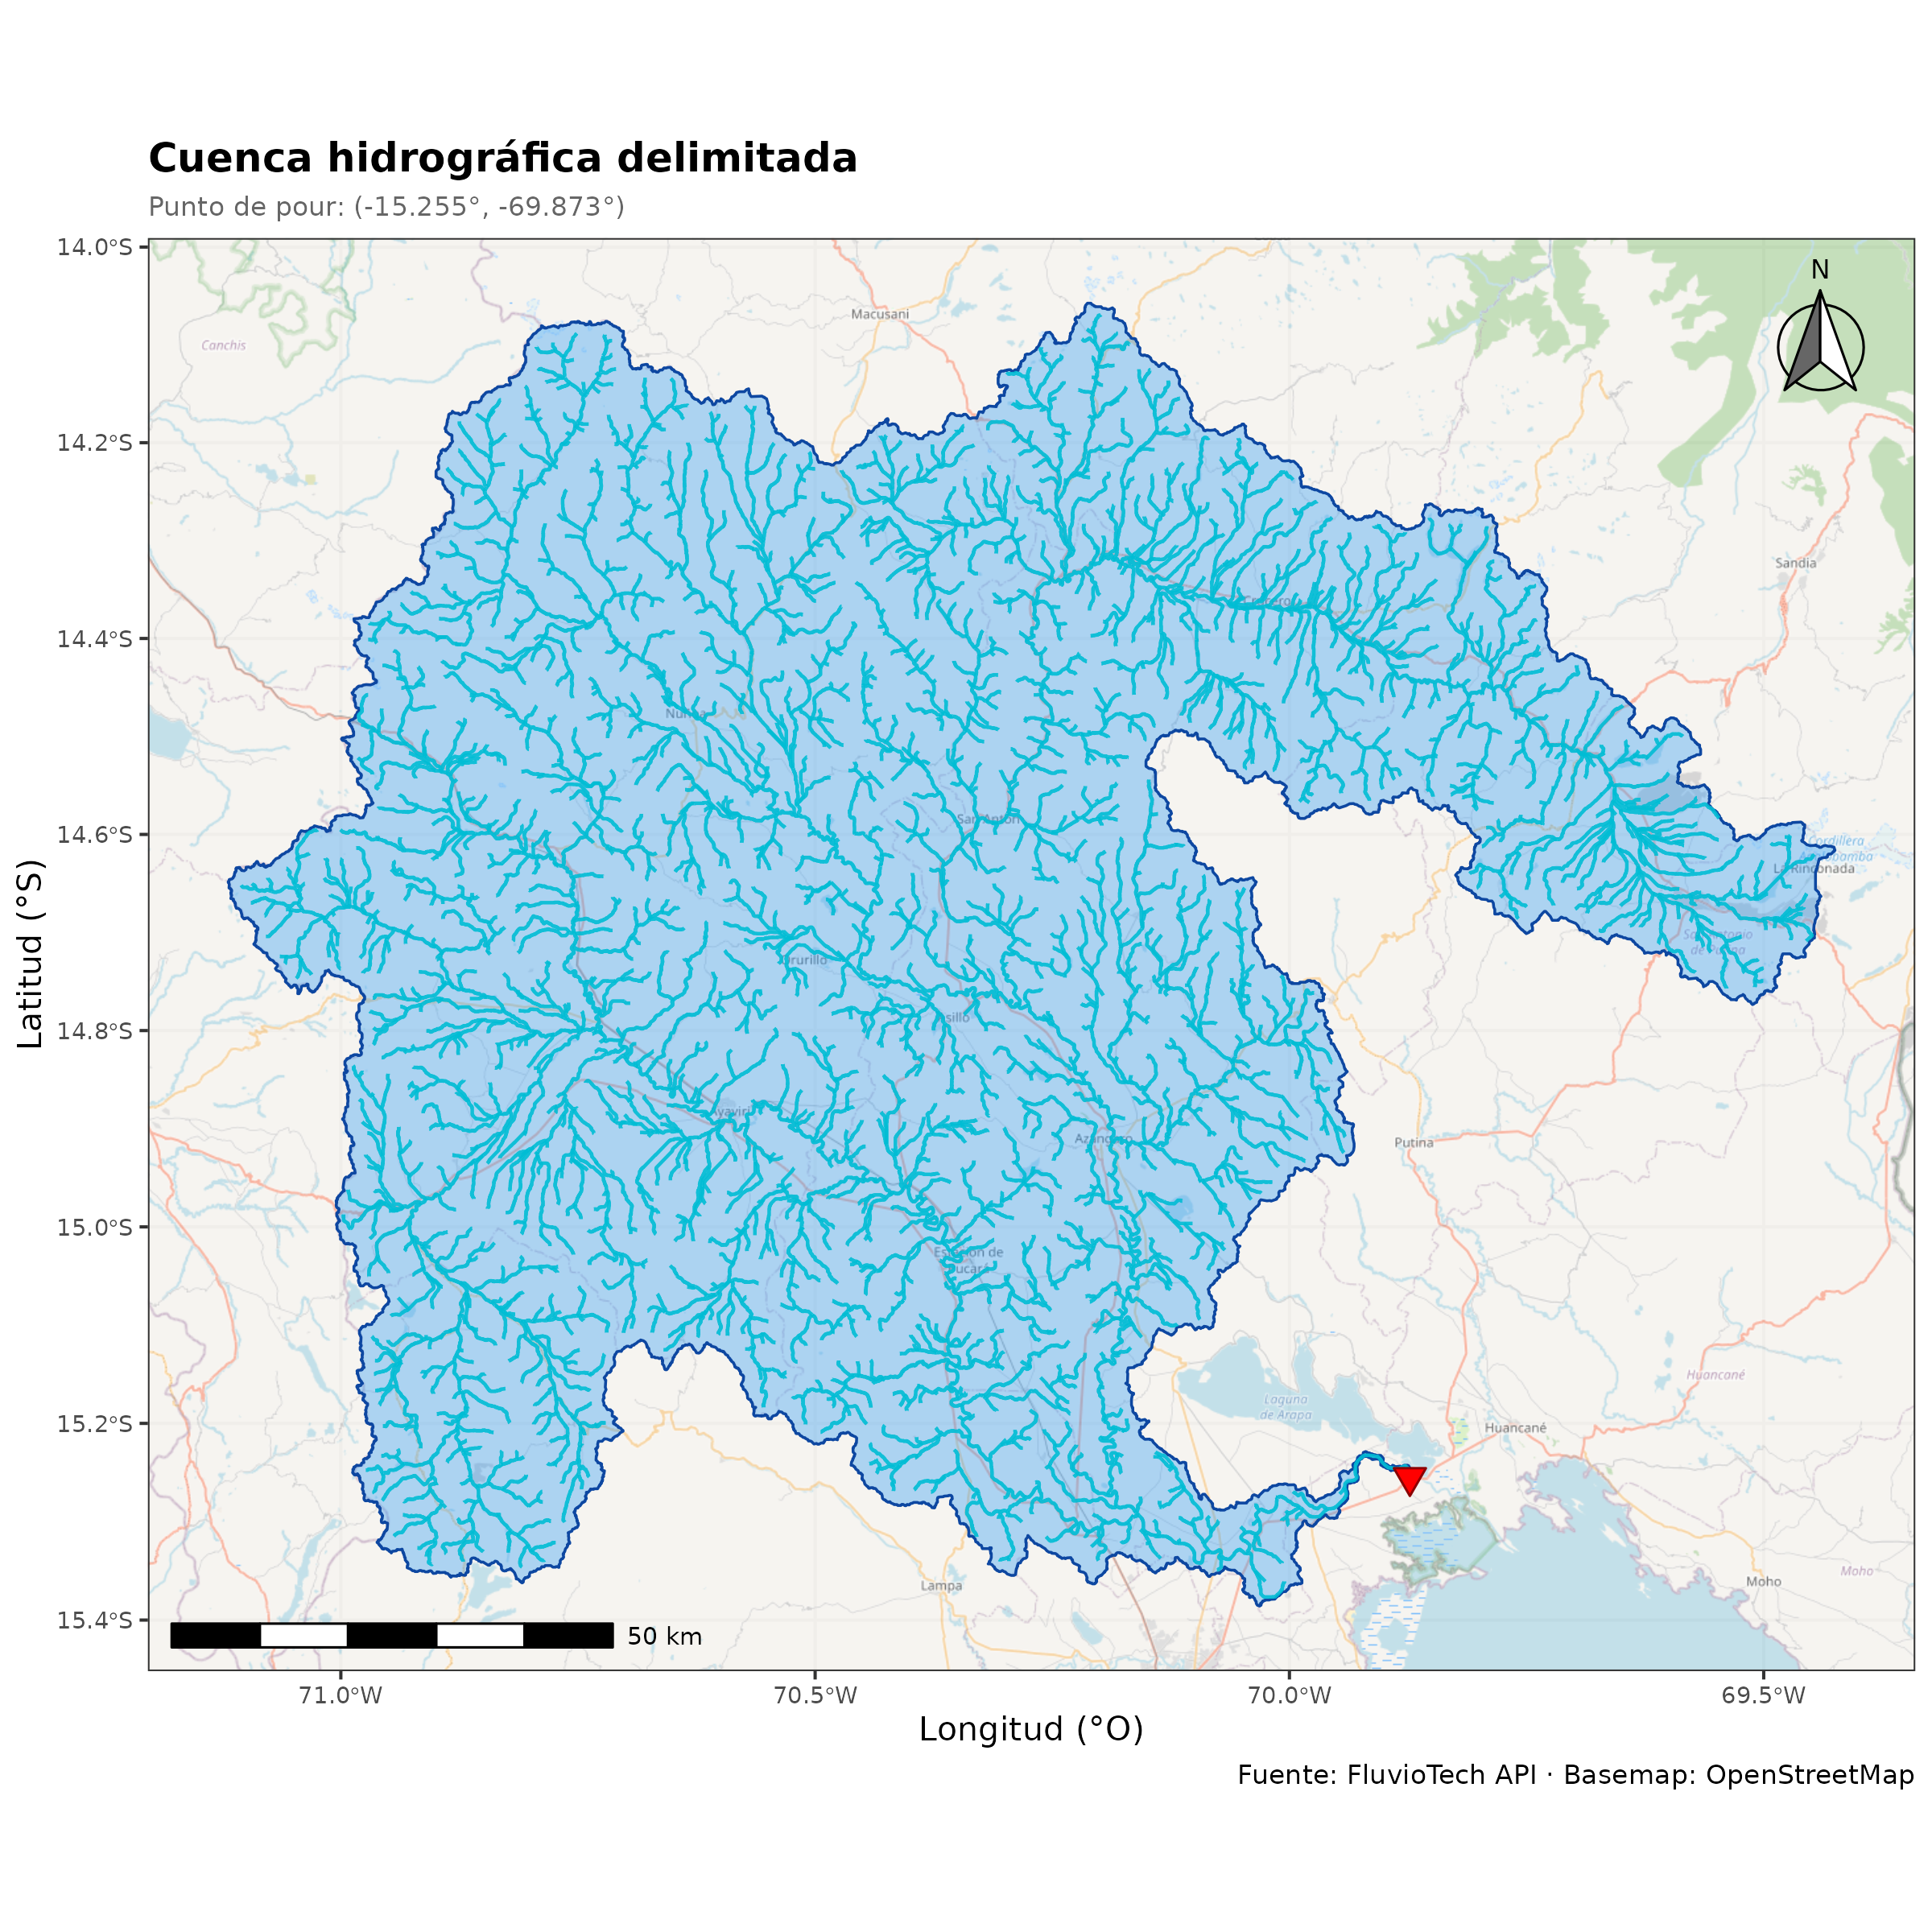
\includegraphics[width=0.92\textwidth]{figures/study_area_ramis.png}%
}{%
\fbox{\parbox[c][0.32\textheight][c]{0.90\textwidth}{\centering
Placeholder for the final study-area map. Replace this box with
\texttt{figures/study\_area\_ramis.png} before submission.}}%
}
\caption{Geographical setting of the Ramis River basin in the
high-Andean Altiplano of southern Peru. The delineated catchment drains
towards Lake Titicaca; the drainage network indicates the main flow
paths represented at catchment scale, and the red marker denotes the
model outlet or pour point used for basin delineation
(15.2550$^{\circ}$S, 69.8730$^{\circ}$W). The map defines the spatial
support used to aggregate gridded precipitation from PISCOp v3.0 and
minimum and maximum air temperature from PISCOt v1.2 into daily
catchment-scale forcings for the lumped rainfall--runoff experiments.}
\label{fig:study-area}
\end{figure*}